\documentclass{article}

% packages
  % basic stuff for rendering math
  \usepackage[letterpaper, top=1in, bottom=1in, left=1in, right=1in]{geometry}
  \usepackage[utf8]{inputenc}
  \usepackage[english]{babel}
  \usepackage{amsmath} 
  \usepackage{amssymb}
  % \usepackage{amsthm}

  % extra math symbols and utilities
  \usepackage{mathtools}        % for extra stuff like \coloneqq
  \usepackage{mathrsfs}         % for extra stuff like \mathsrc{}
  \usepackage{centernot}        % for the centernot arrow 
  \usepackage{bm}               % for better boldsymbol/mathbf 
  \usepackage{enumitem}         % better control over enumerate, itemize
  \usepackage{hyperref}         % for hypertext linking
  \usepackage{fancyvrb}          % for better verbatim environments
  \usepackage{newverbs}         % for texttt{}
  \usepackage{xcolor}           % for colored text 
  \usepackage{listings}         % to include code
  \usepackage{lstautogobble}    % helper package for code
  \usepackage{parcolumns}       % for side by side columns for two column code
  

  % page layout
  \usepackage{fancyhdr}         % for headers and footers 
  \usepackage{lastpage}         % to include last page number in footer 
  \usepackage{parskip}          % for no indentation and space between paragraphs    
  \usepackage[T1]{fontenc}      % to include \textbackslash
  \usepackage{footnote}
  \usepackage{etoolbox}

  % for custom environments
  \usepackage{tcolorbox}        % for better colored boxes in custom environments
  \tcbuselibrary{breakable}     % to allow tcolorboxes to break across pages

  % figures
  \usepackage{pgfplots}
  \pgfplotsset{compat=1.18}
  \usepackage{float}            % for [H] figure placement
  \usepackage{tikz}
  \usepackage{tikz-cd}
  \usepackage{circuitikz}
  \usetikzlibrary{arrows}
  \usetikzlibrary{positioning}
  \usetikzlibrary{calc}
  \usepackage{graphicx}
  \usepackage{caption} 
  \usepackage{subcaption}

  % for tabular stuff 
  \usepackage{dcolumn}

  \usepackage[nottoc]{tocbibind}
  \pdfsuppresswarningpagegroup=1
  \hfuzz=5.002pt                % ignore overfull hbox badness warnings below this limit

% New and replaced operators
  \DeclareMathOperator{\Tr}{Tr}
  \DeclareMathOperator{\Sym}{Sym}
  \DeclareMathOperator{\Span}{span}
  \DeclareMathOperator{\std}{std}
  \DeclareMathOperator{\Cov}{Cov}
  \DeclareMathOperator{\Var}{Var}
  \DeclareMathOperator{\Corr}{Corr}
  \DeclareMathOperator{\pos}{pos}
  \DeclareMathOperator*{\argmin}{\arg\!\min}
  \DeclareMathOperator*{\argmax}{\arg\!\max}
  \newcommand{\ket}[1]{\ensuremath{\left|#1\right\rangle}}
  \newcommand{\bra}[1]{\ensuremath{\left\langle#1\right|}}
  \newcommand{\braket}[2]{\langle #1 | #2 \rangle}
  \newcommand{\qed}{\hfill$\blacksquare$}     % I like QED squares to be black

% Custom Environments
  \newtcolorbox[auto counter, number within=section]{question}[1][]
  {
    colframe = orange!25,
    colback  = orange!10,
    coltitle = orange!20!black,  
    breakable, 
    title = \textbf{Question \thetcbcounter ~(#1)}
  }

  \newtcolorbox[auto counter, number within=section]{exercise}[1][]
  {
    colframe = teal!25,
    colback  = teal!10,
    coltitle = teal!20!black,  
    breakable, 
    title = \textbf{Exercise \thetcbcounter ~(#1)}
  }
  \newtcolorbox[auto counter, number within=section]{solution}[1][]
  {
    colframe = violet!25,
    colback  = violet!10,
    coltitle = violet!20!black,  
    breakable, 
    title = \textbf{Solution \thetcbcounter}
  }
  \newtcolorbox[auto counter, number within=section]{lemma}[1][]
  {
    colframe = red!25,
    colback  = red!10,
    coltitle = red!20!black,  
    breakable, 
    title = \textbf{Lemma \thetcbcounter ~(#1)}
  }
  \newtcolorbox[auto counter, number within=section]{theorem}[1][]
  {
    colframe = red!25,
    colback  = red!10,
    coltitle = red!20!black,  
    breakable, 
    title = \textbf{Theorem \thetcbcounter ~(#1)}
  } 
  \newtcolorbox[auto counter, number within=section]{proof}[1][]
  {
    colframe = orange!25,
    colback  = orange!10,
    coltitle = orange!20!black,  
    breakable, 
    title = \textbf{Proof. }
  } 
  \newtcolorbox[auto counter, number within=section]{definition}[1][]
  {
    colframe = yellow!25,
    colback  = yellow!10,
    coltitle = yellow!20!black,  
    breakable, 
    title = \textbf{Definition \thetcbcounter ~(#1)}
  } 
  \newtcolorbox[auto counter, number within=section]{example}[1][]
  {
    colframe = blue!25,
    colback  = blue!10,
    coltitle = blue!20!black,  
    breakable, 
    title = \textbf{Example \thetcbcounter ~(#1)}
  } 
  \newtcolorbox[auto counter, number within=section]{code}[1][]
  {
    colframe = green!25,
    colback  = green!10,
    coltitle = green!20!black,  
    breakable, 
    title = \textbf{Code \thetcbcounter ~(#1)}
  } 

  \BeforeBeginEnvironment{example}{\savenotes}
  \AfterEndEnvironment{example}{\spewnotes}
  \BeforeBeginEnvironment{lemma}{\savenotes}
  \AfterEndEnvironment{lemma}{\spewnotes}
  \BeforeBeginEnvironment{theorem}{\savenotes}
  \AfterEndEnvironment{theorem}{\spewnotes}
  \BeforeBeginEnvironment{corollary}{\savenotes}
  \AfterEndEnvironment{corollary}{\spewnotes}
  \BeforeBeginEnvironment{definition}{\savenotes}
  \AfterEndEnvironment{definition}{\spewnotes}
  \BeforeBeginEnvironment{exercise}{\savenotes}
  \AfterEndEnvironment{exercise}{\spewnotes}
  \BeforeBeginEnvironment{proof}{\savenotes}
  \AfterEndEnvironment{proof}{\spewnotes}
  \BeforeBeginEnvironment{solution}{\savenotes}
  \AfterEndEnvironment{solution}{\spewnotes}
  \BeforeBeginEnvironment{question}{\savenotes}
  \AfterEndEnvironment{question}{\spewnotes}
  \BeforeBeginEnvironment{code}{\savenotes}
  \AfterEndEnvironment{code}{\spewnotes}

  \definecolor{dkgreen}{rgb}{0,0.6,0}
  \definecolor{gray}{rgb}{0.5,0.5,0.5}
  \definecolor{mauve}{rgb}{0.58,0,0.82}
  \definecolor{lightgray}{gray}{0.93}

  % default options for listings (for code)
  \lstset{
    autogobble,
    frame=ltbr,
    language=C,                           % the language of the code
    aboveskip=3mm,
    belowskip=3mm,
    showstringspaces=false,
    columns=fullflexible,
    keepspaces=true,
    basicstyle={\small\ttfamily},
    numbers=left,
    firstnumber=1,                        % start line number at 1
    numberstyle=\tiny\color{gray},
    keywordstyle=\color{blue},
    commentstyle=\color{dkgreen},
    stringstyle=\color{mauve},
    backgroundcolor=\color{lightgray}, 
    breaklines=true,                      % break lines
    breakatwhitespace=true,
    tabsize=3, 
    xleftmargin=2em, 
    framexleftmargin=1.5em, 
    stepnumber=1
  }

% Page style
  \pagestyle{fancy}
  \fancyhead[L]{Information Theory, Signal Processing}
  \fancyhead[C]{Muchang Bahng}
  \fancyhead[R]{Spring 2024} 
  \fancyfoot[C]{\thepage / \pageref{LastPage}}
  \renewcommand{\footrulewidth}{0.4pt}          % the footer line should be 0.4pt wide
  \renewcommand{\thispagestyle}[1]{}  % needed to include headers in title page

\begin{document}

\title{Information Theory and Signal Processing} 
\author{Muchang Bahng}
\date{Spring 2024}

\maketitle
\tableofcontents
\pagebreak

\section{Introduction}

  \subsection{Channels}

    In a \textit{communication system}, we have a \textit{transmitter} and \textit{receiver}, with \textit{signals} going through a \textit{channel}. Let's briefly define what these terms are, which are pretty much taken verbatim from Shannon's famous paper \cite{shannon}. 

    \begin{figure}[H]
      \centering 
      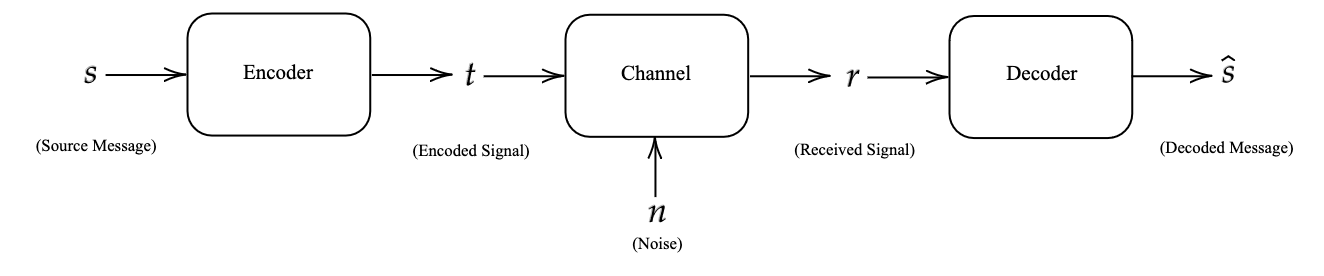
\includegraphics[scale=0.35]{img/channel_diagram.png}
      \caption{A channel diagram. } 
      \label{fig:channel_diagram}
    \end{figure}

    \begin{definition}[Information Source]
      An \textbf{information source} produces a message or sequence of messages to be communicated to the receiving terminal.  
    \end{definition}

    \begin{definition}[Encoder]
      A \textbf{transmitter}, or \textbf{encoder}, operator on the message in some way to produce a signal suitable for transmission over the channel. 
    \end{definition}

    \begin{definition}[Channel]
      The \textbf{channel} is the medium used to transmit the signal from the encoder to the decoder. Some examples of channels are: 
      \begin{enumerate}
        \item A copper wire is a channel connecting one phone to another phone. 
        \item Air is a channel connecting your voice to another's ear. 
        \item Vacuum is a channel connecting an antenna on earth to the Mars rover.  
      \end{enumerate}
    \end{definition}

    \begin{definition}[Decoder]
      The \textbf{decoder}, or the \textbf{receiver} performs the inverse operation of that done by the transmitter, reconstructing the message from the signal. 
    \end{definition}

    \begin{definition}[Destination]
      The \textbf{destination} is the person (or thing) for whom the message is intended.  
    \end{definition}

    All the channels have the property that the received signal is maybe similar, but not identical, to the transmitted signal. This noise is not preferable, and we would ideally like to have perfect communications systems. To reduce this noise, we can improve physical systems (e.g. better insulation in copper wires) or we can improve our systems, such as our encoding/decoding schemes. 

    \begin{example}[Binary Symmetric Channel]
      Given a 1-bit input $x$, there is a certain probability $p$ such that the input is flipped.\footnote{In 2014 disk drives, the standard was that $p$ should not be greater than $10^{-18}$.} This can be sometimes seen in practical applications, e.g. the salt-and-pepper noise in images. 
      \begin{figure}[H]
        \centering 
        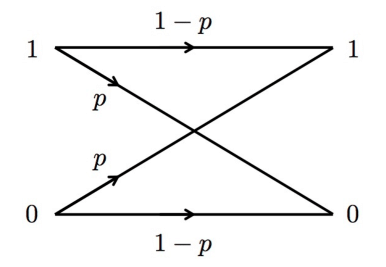
\includegraphics[scale=0.4]{img/binary_symm_channel.png}
        \caption{A simple example of noise. } 
        \label{fig:binary_symm_channel}
      \end{figure}
    \end{example}

  \subsection{Coding Schemes}

    To reduce the probability of $\hat{s} \neq s$, we can devise many schemes of the encoder and decoder. Depending on how much additional information we add, our channel throughput, or \textbf{rate}, becomes lower. 

    \begin{definition}[Parity Encoding]
      Given a string of bits, we can simply add a parity bit. 
      \begin{equation}
        \mathrm{encoder}(x_1, x_2, \ldots, x_n) = x_1, \ldots, x_n, (x_1 \oplus \ldots \oplus x_n)
      \end{equation}
      This has a rate of $n/(n+1)$. 
    \end{definition}

    \begin{definition}[Repetition]
      The encoder can just repeat each bit $k$ times, which we will denote as $R_k$. 
      \begin{equation}
        \mathrm{encoder}(x_1, \ldots, x_n) = x_1, x_1, x_1, x_2, \ldots, x_n
      \end{equation}
      For example, with $k = 3$ we have 
      \begin{lstlisting}
        s = 01101 
        t = 000 111 111 000 111 
        n = 000 100 000 101 000 
        r = 000 011 111 101 111
      \end{lstlisting}
      The decoder then can take the best of 3 to get \texttt{01111}. Note that the second bit had a flip but was fixed, but the second to last bit was an error. We can then compute the probability of these errors with basic computations.\footnote{It turns out that we need $k = 61$ to get a probability of error below $10^{-15}$.} This has a rate of $1/k$. 
    \end{definition}

    We can already predict that these encoding schemes can get quite sophisticated. Here's another one. 

    \begin{definition}[7, 4 Hamming Code]
      Given an input string of bits $\mathbf{s}$, we divide it up into sequences of 4. 
      \begin{equation}
        \mathbf{s}_{i:i+4} = (s_i, s_{i+1}, s_{i+2}, s_{i+3})
      \end{equation}
      Then we can place them in a Venn diagram as shown below and fill out the rest of the three empty spots such that the parity within each circle is $0$. 
      \begin{figure}[H]
        \centering 
        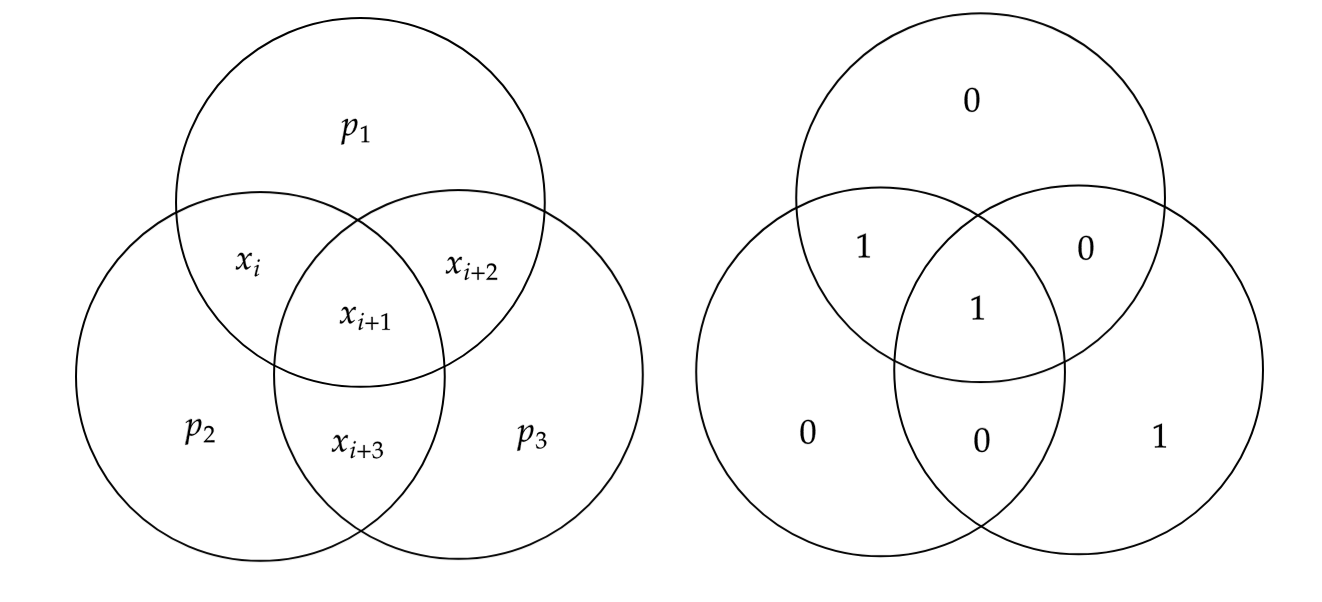
\includegraphics[scale=0.25]{img/hamming_74.png}
        \caption{(7, 4) hamming code visual with example on the right. } 
        \label{fig:hamming_74}
      \end{figure}
      This gives us the encoder. 
      \begin{equation}
        \mathrm{encoder}(x_1, x_2, x_3, x_4) = (x_1, x_2, x_3, x_4, p_1, p_2, p_3)
      \end{equation}
      As for the decoder, we can fill up the Venn diagram with the received bits $r_1, \ldots, r_7$ and then look at the minimum number of bits needed to flip to achieve the same rules we had to fill the inputs out in the Venn diagram. Given any combination of circles that have parity $1$, we can then flip exactly one of the $r_{:}$ to satisfy the rules again (i.e. find the bit that is outside all the valid circles and inside all the invalid circles). This has a rate of $4/7$. 
    \end{definition}

    \begin{theorem}[Conditions for Detection and Correction]
      The (7,4) Hamming code can correct an input if up to 1 bit is flipped in each sequence of 4 bits, but if there are more than 1 bit flip, the decoded sequence will be incorrect. 
    \end{theorem}

    More specifically, the probability of a block error is $21p^2$ on the most significant order and a bit error is $9p^2$. 

    If we look at these different algorithms and plot their rate vs probability of error, we can see some sort of dependency. 

    \begin{figure}[H]
      \centering 
      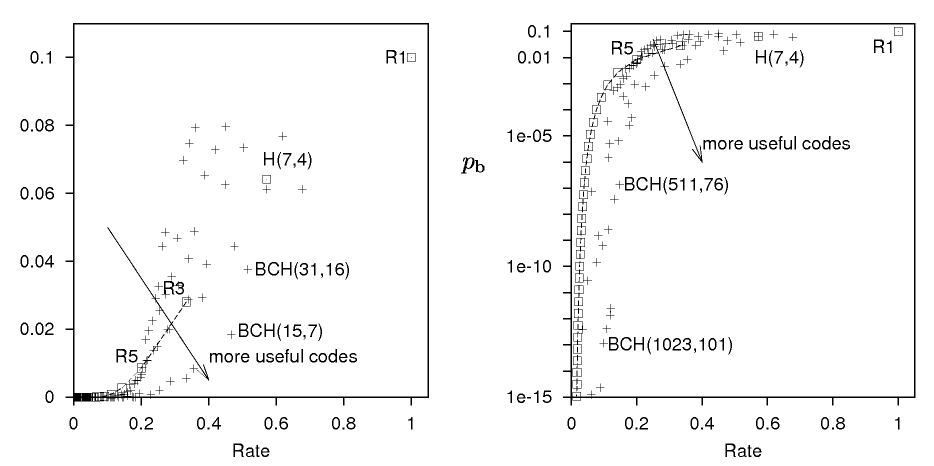
\includegraphics[scale=0.4]{img/rate_vs_error.png}
      \caption{The rate of an encoding/decoding scheme vs probability of bit error.} 
      \label{fig:rate_vs_error}
    \end{figure}

    It was reasonable to assume that we can make schemes that ``hit'' the upper-left portion of the left graph, i.e. we can make schemes that have a low rate (lots of repetition and such) yet still have a low probability of error. The question was how well we can reach the bottom-right corner containing the more useful codes. The general consensus assumed that as the probability of error goes to $0$, the rate must also tend towards $0$, and so we had a boundary that intersected through the origin that separated achievable and non-achievable schemes. However, Claude Shannon remarkably proved that this was not the case, through his \textit{noisy-channel coding theorem}. Rather, we can achieve arbitrarily low probabilities without having to go below some non-zero rate, i.e. this boundary crosses the x-axis at some positive number $C$.  

    \begin{definition}[Capacity]
      $C$ is the \textbf{capacity} of the channel. 
    \end{definition}

    \begin{theorem}[Capacity of Binary Switch Channel]
      The capacity of the BSC with flip probability $f$ is 
      \begin{equation}
        C_{BSC, f} = 1 - H(X), \;\; X \sim \mathrm{Bernoulli}(f)
      \end{equation}
    \end{theorem}

    This means that rather than needing 61 times our input to get past $10^{-15}$ error in the BSC with $f = 0.1$ (which we derive through repetition), we only need 2 disk drives, which is amazing. 

\section{Entropy}

  We have hinted at the fact through Shannon's noisy encoding theorem that there is an optimal way to add redundancies to compress some input. Given a string of random variables $X_1, \ldots, X_n$ generated iid from a $\mathrm{Bernoulli}(p)$ distribution, we want to start to formalize this by introducing a metric to measure the information content of this stochastic process. We motivate the necessity of such a measure using general probability measures and then focus on the discrete case. 

  \subsection{Entropy of Probability Measures}

    First, we want to quantitatively measure the ``surprise'' of an event $E$ happening in a probability space by assigning it a value $H(E)$. We want it to satisfy the following: 
    \begin{enumerate}
      \item $H(E) \geq 0$. The surprisal of any event is nonnegative. 
      \item $H(E) = 0$ iff $\mathbb{P}(E) = 1$. No surprisal is gained from events with probability $1$. 
      \item If $E_1$ and $E_2$ are independent events, then $H(E_1 \cap E_2) = H(E_1) + H(E_2)$. The information from two independent events should be the sum of their informations. 
      \item $H$ should be continuous, i.e. slight changes in probability correspond to slight changes in surprisal. 
    \end{enumerate}

    \begin{definition}[Surprisal]
      Given a probability space $(\Omega, \mathcal{F}, \mathbb{P})$, the \textbf{surprisal}, or \textbf{self-information}, of an event $E \in \mathcal{F}$ is 
      \begin{equation}
        \sigma_\mathbb{P} (E) \coloneqq - \log \mathbb{P}(E)
      \end{equation}
      and the \textbf{expected surprisal} of $E$ is 
      \begin{equation}
        h_\mathbb{P} (E) = \mathbb{P}(E) \sigma_\mathbb{P} (E)
      \end{equation}
    \end{definition}

    Now we can define entropy as the expected surprisal of a random variable, which seems now more motivated and intuitive. 

    \begin{definition}[Entropy]
      Given a probability space $(\Omega, \mathcal{F}, \mathbb{P})$, a $\mathbb{P}$-almost partition is a set family $\mathcal{G} \subset \mathcal{F}$ such that $\mu(\cup_{G \in \mathcal{G}} G) = 1$ and $\mathbb{P}(A \cap B) = 0$ for all distinct $A, B \in \mathcal{G}$ (this is a relaxation of the usual conditions for a partition). The \textbf{entropy} of the subfamily $\mathcal{G}$ is 
      \begin{equation}
        H_\mathbb{P} (\mathcal{G}) \coloneqq \sum_{G \in \mathcal{G}} h_\mathbb{P}(G)
      \end{equation}
      The \textbf{entropy} of the $\sigma$-algebra $\mathcal{F}$ is defined 
      \begin{equation}
        H_\mathbb{P} (\mathcal{F}) = \sup_{\mathcal{G} \subset \mathcal{F}} H_\mathbb{P} (\mathcal{G})
      \end{equation}
      Now the entropy of a random variable $X: (\Omega, \mathcal{F}, \mathbb{P}) \rightarrow (\mathcal{X}, \mathcal{H})$ will induce a measure $\mathbb{P}_X$ on $\mathcal{X}$. Then the entropy of $X$ is defined over this induced measure. 
      \begin{equation}
        H[X] \coloneqq H_{\mathbb{P}_{X}} (\mathcal{H}) = \sup_{G \subset \mathcal{H}} H_{\mathbb{P}_X} (\mathcal{G})
      \end{equation}
    \end{definition}

    Intuitively, this represents the element of surprise of a certain data point, and distributions that have relatively sharp peaks will have lower entropy (since we expect most of the samples to come from the peaks) while uniform distributions have higher entropy. 

  \subsection{Discrete Random Variables}

    With the general version, we can prove the following subdefinition for discrete random variables. 

    \begin{lemma}[Entropy of Discrete RV]
      For a discrete random variable, the entropy reduces to the expectation of the information content. 
      \begin{equation}
        H[X] \coloneqq \mathbb{E}_X [-\ln{p(X)}] = -\sum_{x \in \mathcal{X}} \mathbb{P}(X = x) \ln{\mathbb{P}(X = x)}
      \end{equation}
      where we use $p(x)$ as the PMF. 
    \end{lemma}
    \begin{proof}
      TBD. Since we are working with the power set, ...
    \end{proof}

    In Shannon's famous paper \cite{shannon}, he talks first on discrete channels, focusing on examples of transmitting languages through n-gram models as ``higher order approximations'' of language.\footnote{In fact, this is where n-gram models were first referenced.} This is an ergodic Markov chain with some stationary distribution. 

    He then asks whether we can have some sort of measure on how much information is produced by the process, or at what rate the information is produced? Borrowing his terminology, if we have some measure $H(p_1, \ldots, p_n)$, he states that it is reasonable to require the following properties, which are slightly different than ours. $H$ should measure the uncertainty of the outcome. 
    \begin{enumerate}
      \item $H$ should be continuous in $p_i$.  
      \item If all $p_i$ are equal, then $H$ should be a monotonic increasing function of $n$. With equally likely events there is more choice, or uncertainty, when there are more possible events. 
      \item If a choice is broken down into two successive choices, the original $H$ should be a weighted sum of the individual values of $H$. For example, the uncertainty of both distributions should be the same. 
      \begin{center}
        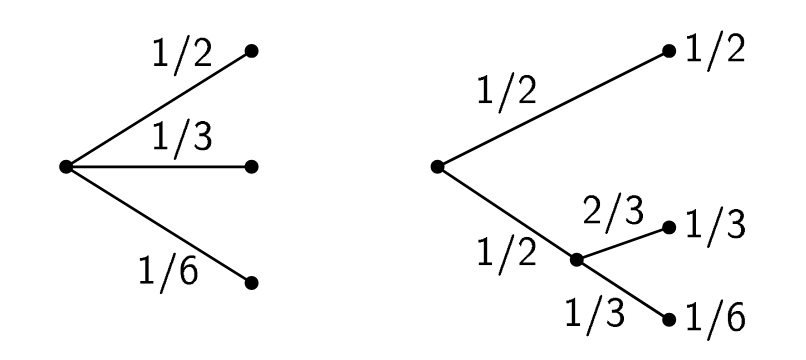
\includegraphics[scale=0.6]{img/same_entropy.png}
      \end{center}
      That is, 
      \begin{equation}
        H\big( \frac{1}{2}, \frac{1}{3}, \frac{1}{6} \big) = H \big(\frac{1}{2}, \frac{1}{2} \big) + \frac{1}{2} H \big( \frac{2}{3}, \frac{1}{3} \big)
      \end{equation}
    \end{enumerate}
    Which then leads to the definition of entropy above. Note the following properties. 

    \begin{theorem}[Bounds on Entropy]
      $H$ is bounded by $0$ and $1$, attaining its minimum if and only if all the $p_i$ but one are $0$. It attains its maximum if $p$ is uniform. 
    \end{theorem}

    \begin{example}[Bits]
      Given $X \sim \mathrm{Bernoulli}(p)$, if we observe a value of $1$, then we have received $\log_2 \big( \frac{1}{p} \big)$ bits of information. 
    \end{example}

    Now Shannon's claim is that this information content is the optimal encoding length that we should aim for. For example, given $p = 0.9$, then a $0$ has 3.32 bits of information content and a $1$ has 0.15 bits. This means that $0$'s, which occur infrequently, should be encoded with longer strings and $1$ with shorter strings.   

    \begin{exercise}[Weighing Problem]
      You are given 12 balls, all equal in weight except for one that is either heavier or lighter. Design a strategy to determine which is the odd ball \textit{and} whether it is heavier or lighter in as few uses of the balance as possible. 
    \end{exercise}

    \begin{proof}
      We can tackle this by looking at the first action. We can choose to weigh $n$ vs $n$ balls for $n = 1, \ldots, 6$. Shannon would advise you to choose such that we maximize our entropy, or expected information gain. Let's go through them one at a time. Our three outcomes for all scenarios are $A$ (left is lighter), $B$ (both equal), and $C$ (right is lighter). 
      \begin{enumerate}
        \item 6 v 6. The probability distribution is $(A, B, C) = (1/2, 0, 1/2)$ and so the entropy is $H = 1$ bit. 
        \item 5 v 5. The distribution is $(5/12, 1/6, 5/12)$ giving us $H = 1.48$ bits. 
        \item 4 v 4. The distribution is $(1/3, 1/3, 1/3)$ giving us $H = 1.58$ bits. 
        \item We go on. 
      \end{enumerate}
      We already know that entropy must be maximized in the uniform distribution, so it is best to choose 4 v 4. This is indeed the correct first step. 
      
    \end{proof}

  \subsection{Joint and Conditional Entropy}

    \begin{definition}[Joint, Conditional Entropy]
      We can define the joint entropy and conditional entropy between two discrete random variables $X, Y$ as 
      \begin{align*}
        H(X, Y) & = \mathbb{E}_{X \times Y} [-\log p(x, y)] = \sum_{x, y \in \mathcal{X}, \mathcal{Y}} p(x, y) \cdot - \log p(x, y) \\
        H(X \mid Y) & = \mathbb{E}_{X \times Y} [- \log p(x \mid y)]  = \sum_{x, y \in \mathcal{X}, \mathcal{Y}} p(x, y) \cdot - \log p(x \mid y )
      \end{align*}
    \end{definition}

    \begin{theorem}[Joint Entropy]
      The uncertainty of a joint event is less than or equal to the sum of the individual uncertainties, with equality achieved only if the events are independent. 
      \begin{equation}
        H(X, Y) \leq H(X) + H(Y)
      \end{equation}
    \end{theorem}

    Another property is that any change towards ``equalization'' of the probabilities $p_i$ increases $H$. Since we don't have a method of measuring how close to the uniform distribution, we will return back to this after defining the KL divergence.  

    \begin{theorem}[Conditional Entropy]
      The joint entropy is the entropy of $X$ plus the conditional entropy of $Y$ given $X$. 
      \begin{equation}
        H(X, Y) = H(X) + H(Y \mid X) = H(Y) + H(X \mid Y)
      \end{equation}
    \end{theorem}

    \begin{theorem}[Conditioning Never Decreases Uncertainty]
      Since 
      \begin{equation}
        H(X) + H(Y) \geq H(X, Y) = H(X) + H(Y \mid X)
      \end{equation}
      we have $H(Y) \geq H(Y \mid X)$. That is, the uncertainty of $Y$ is never increased by the knowledge of $X$. 
    \end{theorem}

    In fact, the amount of uncertainty that decreases when conditioning has a well known name. 

    \begin{definition}[Mutual Information]
      The \textbf{mutual information} between random variables $X, Y$ is the decrease in entropy when we condition $X$ by $Y$. 
      \begin{equation}
        I(X ; Y) = H(X) - H(X \mid Y) = H(Y) - H(Y \mid X)
      \end{equation}
      This can be conditioned on another random variable $Z$. 
      \begin{equation}
        I(X ; Y \mid Z) = H(X \mid Z) - H(X \mid Y, Z) = H(Y \mid Z) - H(Y \mid X, Z)
      \end{equation}
    \end{definition}

    The entropy also demonstrates the average length (if base is $2$) number of bits required to transmit the state of a random variable. 

  \subsection{Differential Entropy}

    \begin{definition}[Differential Entropy]
      For a continuous random vector, the \textbf{differential entropy} is defined 
      \begin{equation}
        H[\mathbf{X}] = - \int p(\mathbf{x}) \ln{p(\mathbf{x})} \,d\mathbf{x}
      \end{equation}
    \end{definition}

  \subsection{Kullback Leibler Divergence}

    The \textbf{relative entropy}, or \textbf{Kullback-Leibler divergence}, of distributions $p(x)$ and $q(x)$ is defined 
    \begin{align*}
      \mathrm{KL}(p || q) & \coloneqq - \int p(\mathbf{x}) \, \ln{q(\mathbf{x})} \,d\mathbf{x} - \bigg( - \int p(\mathbf{x}) \, \ln{p(\mathbf{x})} \,d\mathbf{x} \bigg) \\
      & = - \int p(\mathbf{x}) \, \ln \bigg( \frac{q(\mathbf{x})}{p(\mathbf{x})} \bigg) \,d\mathbf{x} 
    \end{align*}
    We can show that this quantity is always greater than or equal $0$ by Jensen's inequality using the fact that $-\ln(x)$ is concave
    \begin{equation}
      \int p(\mathbf{x}) \, -\ln \bigg( \frac{q(\mathbf{x})}{p(\mathbf{x})} \bigg) \,d\mathbf{x} \geq -\ln \int p(\mathbf{x}) \, \frac{q(\mathbf{x})}{p(\mathbf{x})} \,d\mathbf{x} = -\ln \int q(\mathbf{x}) \,d\mathbf{x} = -\ln(1) = 0
    \end{equation}
    and it is precisely $0$ if $p = q$, so it behaves similarly to a metric. However, it isn't exactly since it is not symmetric. 

    Let's demonstrate how entropy and the KL divergence applies to maximum likelihood estimation. Suppose that iid samples $\mathcal{D} = \{(x^{(n)}, y^{(n)}\}$ are given in a regression problem. Let $P^\ast = (X, Y)$ be the true data generating function. Then, we want to compute an approximation of $P^\ast$ with $P_\theta$, where $P_\theta$ is some parameterized distribution. The negative log likelihood of the $y$'s being generated is 
    \begin{equation}
      \ell(\theta) = \frac{1}{N} \sum_{n=1}^N \log P_\theta (y_i \mid x_i)
    \end{equation}
    which asymptotically converges to 
    \begin{equation}
      \mathbb{E}_{P^\ast} [ -\log P_\theta (y_i \mid x_i)] = \mathrm{KL}(P^\ast || P) + H[P^\ast]
    \end{equation}
    and since the entropy is constant, this is equivalent to minimizing the KL divergence between $P$ and $P^\ast$. 

    We assume that the $y^{(n)}$'s come from a conditional distribution $P_{\theta, x_i}$, where the parameters of the distribution is $\theta$ and $x_i$ 

\bibliographystyle{plain}
\bibliography{./bibfile}
\end{document}
